

Let us consider a circle of mass M in the $(x,y)$-plane of radius $R$ centered at the origin.
Let us consider a point $P$ of coordinates $(x_P,y_P,z_P)$ 
%(because of the axisymmetry we can always rotate the system so as to put the $M$ point on the $x$-axis).

FIGURE


We are considering a small element of the ring of mass $\delta m$ (with $\oint dm = M$). 
The contribution of this element to the field is
\[
\delta \vec{g} = \frac{{\cal G} \delta m}{d^2} \vec{e}_{MP}
\]

In what follow we sent the linear density to $\rho=10^6~\si{\kg\per\meter}$ and 
the radius of the circle to $R=1.123$

%----------------------------------------------------------------
\subsection*{Case 1: $P$ is above the center of the circle}

In this case:
\[
d=\sqrt{R^2 + z_P^2}
\]
and because of symmetry we know that the resulting 
gravity components $g_x$ and $g_y$ will be zero.

\begin{center}
\includegraphics[width=7cm]{python_codes/fieldstone_132/results/case1/setup.pdf}
\end{center}

For the mass $\delta m$ the contribution on the $z$-axis
is given by 
\[
\delta g_z = \frac{{\cal G} \delta m}{R^2+z_P^2} \cos\theta 
\] 
We see that 
\[
\cos\theta = \frac{z_P}{\sqrt{R^2+z_P^2}}
\]
so that
\[
\delta g_z = \frac{{\cal G} \delta m}{R^2+z_P^2}\frac{z_P}{\sqrt{R^2+z_P^2}}
\] 
By integrating this expression for the entire circle we find:
\[
g_z=\frac{{\cal G} M z_P}{(R^2+z_P^2)^{3/2}}
\]
See also video \url{https://www.youtube.com/watch?v=q5EWLNdv_pE}

\begin{center}
\includegraphics[width=7cm]{python_codes/fieldstone_132/results/case1/gz.pdf}\\
{\captionfont Vertical component of the gravity field as a function of $z$, 
for various circle resolution, plotted against the analytical solution.}
\end{center}




%----------------------------------------------------------------
\subsection*{Case 2: $P$ is in the plane circle}


\begin{center}
\includegraphics[width=5.7cm]{python_codes/fieldstone_132/results/setup.pdf}
\end{center}

\begin{center}
\includegraphics[width=5.7cm]{python_codes/fieldstone_132/results/gx.pdf}
\includegraphics[width=5.7cm]{python_codes/fieldstone_132/results/gx2.pdf}
\includegraphics[width=5.7cm]{python_codes/fieldstone_132/results/gx3.pdf}
\end{center}
